\chapter{Quantifying dynamism in compiler framework pattern rewriting}
\label{chap:dynamism-pattern-rewriting}

%% Introduction
% Hook
A key difference between the Python and C++ runtimes is their degree of dynamism.
% Argument
\ac{mlir}'s C++ runtime incurs overhead when dynamically dispatching functions (\autoref{fig:narrative}, \circledbase{pairedThreeLightGreen}{3}), which is worsened by prohibiting ahead-of-time performance optimisations. In contrast, almost every bytecode operation evaluated by the Python interpreter is dynamic, each incurring an overhead.
As such, we expect the difference in performance between language runtimes (\autoref{fig:narrative}, \circledbase{pairedFourDarkGreen}{4}) to be smaller for more dynamic workloads.
% Link
In this chapter, we quantify this difference by examining simple examples within static and dynamic language runtimes. We then apply this information to understand the difference in performance between pattern rewriting workloads using xDSL and \ac{mlir} through the lens of overhead incurred by dynamism.


\section{Cost of dynamic dispatch}
\label{chap:dynamism-pattern-rewriting-dispatch}

%% Introduce the issue, and where it is in the micro-benchmark
% Hook
In static languages such as C++, the exact address of many function calls can be resolved at compile time. In contrast, dynamic languages such as Python must resolve the address of each function call at runtime, incurring an overhead.
% Also optimisation boundary and stuff
% Argument
However, the address of some function calls can only be known at runtime, for example as a result of object polymorphism. This address then must be resolved during execution by the language runtime in both static and dynamic languages. Furthermore, this information being known only at runtime presents and optimisation boundary, precluding common rewrites such as function inlining which contribute to the performance of ahead-of-time compiled languages.
Driesen and H\"olzle quantify the former and acknowledge the latter cost in their work ``The Direct Cost of Virtual Function Calls in C++'' \cite{driesenDirectCostVirtual1996}, which found that C++ programs spent a median of $5.2\%$ of their time in dispatch code.
We argue further that the difference between static and dynamic languages is reduced for highly dynamic workloads with insufficient information to resolve function addresses ahead of time.
% Link
We justify this by examining the mechanisms of dynamic dispatch in Python and C++, and contrasting them through both synthetic examples and our micro-benchmark suite.

% Hook
% Argument
C++ uses a \ac{vtable} mechanism for method polymorphism, a lookup table which is accessed at runtime through pointer indirection to retrieve the address for the virtual function implementation. In contrast, Python stores methods and attributes in the \mintinline{text}{__dict__} object attribute which is searched at runtime, checking parent classes if needed. While both use indirection for dynamic dispatch, Python's approach enables more dynamic behaviour like runtime meta-programming but comes with higher performance costs compared to C++'s more efficient \ac{vtable} system.
% Link
We can quantify the performance overhead of this \ac{vtable} mechanism through a synthetic example (Listing \ref{listing:impact-dispatch}).


\begin{figure}[H]
    \centering
    \begin{subfigure}[b]{0.45\textwidth}
       \centering
        \begin{minted}[fontsize=\scriptsize,escapeinside=££]{text}
class Base {
public:
    int func(int a, int b) { £\circledbase{pairedTwoDarkBlue}{\scriptsize{1}}£
        return a - b;
    }
    __attribute__((noinline))
    int uninlinedFunc(int a, int b) { £\circledbase{pairedThreeLightGreen}{\scriptsize{2}}£
        return a - b;
    }
    virtual int virtualFunc(int a, int b) { £\circledbase{pairedFourDarkGreen}{\scriptsize{3}}£
        return a - b;
    }
};

class Derived : public Base {
public:
    int virtualFunc(int a, int b) override {
        return b - a;
    }
};
        \end{minted}
        \scriptsize{\vspace{1em}}
        \captionsetup{name=Listing}
        \caption{Method definitions.}
        \label{listing:impact-dispatch-definition}
    \end{subfigure}
    \hfill
    \begin{subfigure}[b]{0.45\textwidth}
        \centering
        \begin{minted}[breakanywhere,fontsize=\scriptsize,escapeinside=££]{text}
#include <stdlib.h>

int main(int argc, char *argv[]) {
    // Values known only at runtime
    int a = atoi(argv[1]), b = atoi(argv[2]), c = atoi(argv[3]);

    // Setup
    int result = 0;
    Base baseObj;
    Derived derivedObj;
    Base* polyObj = c > 0 ? &baseObj : &derivedObj; £\circledbase{pairedOneLightBlue}{\scriptsize{4}}£

    // Function invocations
    result += baseObj.func(a, b);
    result += baseObj.uninlinedFunc(a, b);
    result += polyObj->virtualFunc(a, b);

    return result;
}
        \end{minted}
        \captionsetup{name=Listing}
        \caption{Method invocations.}
        \label{listing:impact-dispatch-invocation}
    \end{subfigure}
    \vspace{1em}
    \captionsetup{name=Listing}
    \caption{Synthetic example of direct and dynamic method dispatch in C++.}
    \label{listing:impact-dispatch}
\end{figure}

% Hook
Our experiment
% Argument
% Link

\begin{figure}[H]
    \centering
    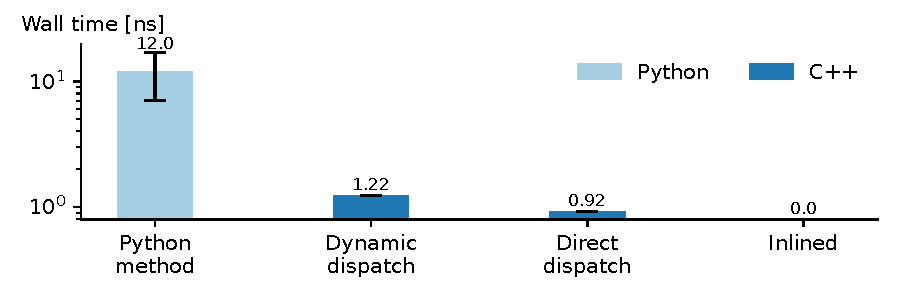
\includegraphics[width=0.75\textwidth]{images/impact_dynamism/dispatch.pdf}
    \caption{Dynamic dispatch in C++ incurs a $30\%$ overhead in C++ method invocation, but remains an order of magnitude more performant than CPython 3.10 method invocation.}
    \label{figure:impact-dispatch}
\end{figure}


% % Hook
From this experiment, we can see taht
% % Argument
The pointer dereference cost is small but non-negligible.
The hidden optimisation opportunities are bigger.
Python is much slower, and a two-step process (LOAD\_METHOD + CALL\_METHOD), where LOAD\_METHOD is slow.
% %% Where does this occur?
% % Hook
%% Introduction
% Hook
In addition to the direct overhead incurred by dynamism in static languages, runtime information precludes ahead-of-time optimisations which contribute to the difference in performance between static and dynamic languages.
% Argument
% Not categorised, since "indirect" cost by diesen and holzer
% Examples of how
% Link


This behaviour
% Argument
% Link
In other cases, \ac{mlir} is implemented to avoid this overhead. For example, the \mintinline{text}{TypeID::get<Traits>} function uses template meta-programming to monomorphise the generic function calls. However, this approach is only applicable when there is sufficient information at runtime.




\section{Run-time type information}
\label{chap:dynamism-pattern-rewriting-rtti}

%% Introduce the issue
% Hook
In a ``A history of C++: 1979--1991'', Stroustop states that the original C++ design ``deliberately didn't include [mechanisms] for run-time type identification [as] they were almost always misused.'' \cite{stroustrupHistory197919911996}.
% Argument
Support for this functionality was later added in C++98 \cite{internationalorganizationforstandardizationISOIEC148821998}, including support for \texttt{dynamic\_cast}s checked a runtime, and getting the \texttt{typeid} of a polymorphic object. However, this incurs a runtime cost \cite{goldthwaite2006technical}, and is brittle in the objects to which it can be applied. A such, LLVM reimplements a subset of this functionality, providing the \texttt{dyn\_cast} method and \texttt{TypeID} data structure, aiming to ``strike a balance between performance and the setup required to enable its use'' \cite{mlirteamMLIRCodeDocumentation}.
This is another example of dynamic behaviour, which we again argue incurs additional runtime overhead and precludes optimisations in static languages, closing the gap with dynamic ones.
% Link
As before, we justify this be examining the details of this mechanism, using both synthetic examples and our micro-benchmark suite.

%% Graph
\begin{figure}[H]
    \centering
    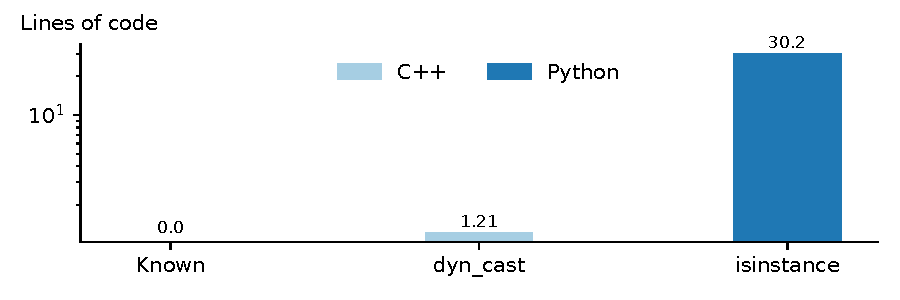
\includegraphics[width=0.75\textwidth]{images/impact_dynamism/dynamic_cast.pdf}
    \caption{.}
    \label{figure:impact-rtti}
\end{figure}

%% Experimental results
% Hook
These results show that LLVM's \ac{rtti} implementation.
% Argument
Approximately one third of Python's runtime is as a result of its method invocation overhead, quantified as $10$ns in the previous experiment. Despite this, the type checking implementation . This comes as a result of CPython's \texttt{PyObject\_IsInstance} implementation,
% Duck typing avoids need for type checking -- asserts elided by -O0
However, Python's duck typing
% Where is this present in micro-benchmarks
This synthetic example can be seen in the trait checking micro-benchmark, demonstrating its relevance to user-extensible compiler infrastructure. In \ac{mlir}, LLVM's \mintinline{c++}{TypeID} \ac{rtti} infrastructure is used to compare traits, constrasting Python using \texttt{isinstance} checks (\autoref{listing:ubenchmark-trait-checks-both}).
% Link




% \section{Object data access}
% \label{chap:dynamism-pattern-rewriting-access}
% __slots__ and polymorphism stuff








\section{Dynamism in pattern rewriting}
\label{chap:dynamism-pattern-rewriting-summary}

%% Introduction

%% Something about RTTI

%% Count up vtable invocations in C++ to argue about dynamic dispatch
% Hook
In addition to quantifying the performance of \ac{vtable} accesses, we can also estimate the number of dynamic calls made for a running workload.
% Argument
In the ARM instruction set, direct and indirect calls \cite{armlimitedARMCortexRSeries}
``Because the branch destination is PC-relative, it can be determined exactly at an early stage of the pipeline''. This means that direct calls are more performant, and as such efficient compilers only use indirect calls where address information is not known ahead of time: dynamic control flow.
Using the \texttt{perf} tool, we can leverage hardware performance counters to total the number of indirect calls made.
% Link

%% Estimate lower bound for cost of dynamism

%% Summary
